\documentclass[cjk]{beamer}
\usepackage{CJK}
\usepackage{amsmath}
\usepackage{graphicx}
\usepackage{float}
\usepackage{fancyhdr}
\usepackage{algorithm}
\usepackage{algpseudocode}
\usetheme{CopenHagen}
\usecolortheme{seagull}
\begin{document}
\begin{CJK*}{UTF8}{gbsn}
\title{算分回顾 03-14}
\author{黄道吉-1600017857}
\institute{元培学院}
\date{\today}

\begin{frame}
    \titlepage
\end{frame}

\begin{frame}
    \frametitle{目录}
    \tableofcontents
\end{frame}

\section{recap}
  \begin{frame}
    \frametitle{recap}
    \begin{itemize}
      \item 最近点对
        \begin{itemize}
          \item 预处理降低计算复杂度
          \item 设计相应的数据结构
        \end{itemize}
      \item 分治选择算法及其复杂度估计
    \end{itemize}
  \end{frame}

\section{convolution}
  \subsection{introduction}
    \begin{frame}
      \frametitle{vector operation}
      \begin{itemize}
        \item 向量和 $a + b = (a_0 + b_0,..., a_{n - 1} + b_{n - 1})$
        \item 内积   $a \* b = (a_0b_0 + ... + a_{n - 1}b_{n - 1})$
        \item 卷积
        $a \* b = (c_0, ..., c_{2n - 2})$ 其中 $c_k = \sum\limits_{i + j = k, i, j < n} a_ib_j$
        \item
        \begin{equation*}
          \left(
          \begin{array}{ccccc}
            a_0b_0 & a_0b_1 & \dots & a_0b_{n - 2} & a_0b_{n - 1} \\
            a_1b_0 & a_1b_1 & \dots & a_1b_{n - 2} & a_1b_{n - 1} \\
            \dots & \dots & \dots & \dots & \dots \\
            a_{n - 1}b_0 & a_{n - 1}b_1 & \dots & a_{n - 1}b_{n - 2} & a_{n - 1}b_{n - 1} \\
          \end{array}
          \right)
        \end{equation*}
      \item 可以看作两个多项式相乘之后的各项系数
        \begin{equation*}
          \begin{split}
          C(x) &= A(x)B(x) \\
          A(x) &= \sum_0^{m - 1}a_ix^i \quad B(x) = \sum_0^{n - 1}b_ix_i
        \end{split}
        \end{equation*}
      \end{itemize}
    \end{frame}

    \begin{frame}
      \frametitle{convolution computation}
      \begin{itemize}
        \item 直接计算: O($n^2$)
        \item 快速算法
          \begin{itemize}
            \item 选择$x_1, ..., x_{2n}$, 求出$A(x_j)$和$B(x_j)$
            \item 计算$C(x_j) = A(x_j)B(x_j)$
            \item 利用插值算法, 求出$C(x)$
            \item 下面只需要说明可以在$\Theta(n\log n)$时间内对多项式求值, 反解出多项式
              \newline
              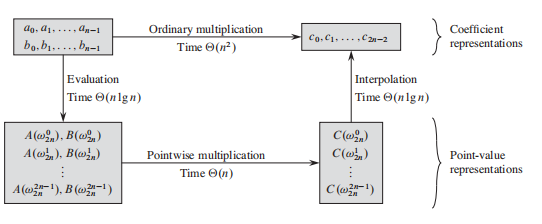
\includegraphics[scale = 0.5]{1.png}
          \end{itemize}
      \end{itemize}
    \end{frame}

  \subsection{prerequisites}
    \begin{frame}
      \frametitle{interpolation}
      \begin{itemize}
        \item 可以用点值对表示多项式: 给定$n - 1$次多项式在$n$个点的取值, 可以唯一确定这个多项式, 反解出系数只需计算$a = V(x_0, ..., x_{n - 1})^{-1}y$即可, 但这是$O(n^3)$的算法
          \newline
          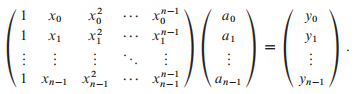
\includegraphics[scale = 0.75]{4.png}
        \item 拉格朗日插值可以做到用$\Theta(n^2)$的时间计算系数向量.
          \begin{equation*}
            A(x) = \sum_{k = 0}^{n - 1}y_k \frac{\prod\limits_{j \neq k}(x - x_j)}{\prod\limits_{j \neq k}(x_k - x_j)}
          \end{equation*}
      \end{itemize}
    \end{frame}

    \begin{frame}
      \frametitle{complex roots of unity}
      \begin{itemize}
        \item 1的单位根表示为$\omega^n = 1$
        \item 在复平面上的表示
          \newline
          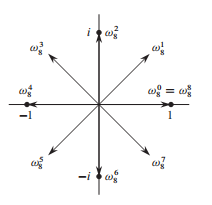
\includegraphics[scale = 0.7]{3.png}
          \newline
        \item 2n次方根的平方是n次方根, 即$(\omega_{2n}^k)^2 = \omega_n^k$
      \end{itemize}
    \end{frame}

    \begin{frame}
      \frametitle{DFT and FFT}
      \begin{itemize}
        \item 假定一个多项式$A(x) = \sum\limits_{i = 0}^{m - 1}a_ix^i$以系数向量的形式给出$a = (a_0, ..., a_{n - 1})$, 定义
        \begin{equation*}
          y_k = A(\omega_n^k) = \sum_{j = 0}^{n - 1} a_j\omega_n^{kj}
        \end{equation*}
        则$y = (y_0, ..., y_{n - 1}) = DFT_n(a)$称为系数向量的离散傅里叶变换
      \end{itemize}
    \end{frame}

    \begin{frame}
      \frametitle{DFT and FFT}
      \begin{itemize}
        \item 通过FFT可以在$\Theta(n\log n)$时间内计算出DFT, 反解出系数向量
        \item 将多项式按照奇偶项分成两个n / 2次多项式
          \begin{equation*}
            \begin{split}
              A^{[0]}(x) &= a_0 + ... + a_{n - 2}x^{n / 2 - 1}, \\
              A^{[1]}(x) &= a_1 + ... + a_{n - 1}x^{n / 2 - 1}.
            \end{split}
          \end{equation*}
          则有
          \begin{equation*}
            A(x) = A^{[0]}(x^2) + xA^{[1]}(x^2)
          \end{equation*}
      \end{itemize}
    \end{frame}

    \begin{frame}
      \frametitle{DFT and FFT}
      \begin{itemize}
        \item $A(x) = A^{[0]}(x^2) + xA^{[1]}(x^2)$
        \item 这样对n次多项式的求值转化为对两个n / 2次多项式的求值
        \item 并且 $(\omega^0_n)^2, ..., (\omega^{n - 1}_n)^2$正好是1的n / 2次方根, 正好得到规模减小的原问题
        \item 合并子问题解的过程可以在$O(n)$时间内完成, 也可以利用单位根的性质做优化.
      \end{itemize}
    \end{frame}
  \subsection{FFT and DFT$^{-1}$}
    \begin{frame}
      \frametitle{FFT pseudo-code}
          \begin{algorithm}[H]
            \caption{Recursive-FFT(a)}
            \begin{algorithmic}[1]
              \State n = a.$length$
              \If{n == 1} \Return{a}
              \EndIf
              \State $\omega_n = e^{2\phi i / n} \quad \quad \omega = 1$
              \State $a^{[0]} = (a_0, ..., a_{n - 2}) \quad a^{[1]} = (a_1, ..., a_{n - 1})$
              \State $y^{[0]} = Recursive-FFT(a^{[0]}) \quad y^{[1]} = Recursive-FFT(a^{[1]})$
              \For{$k = 0 \to n / 2 - 1$}
                \State $y_k$ = $y^{[0]}_k + \omega y^{[1]}_k$
                \State $y_{k + n / 2}$ = $y^{[0]}_k - \omega y^{[1]}_k$
                \State $\omega = \omega \omega_n$
              \EndFor
              \State \Return{y}
            \end{algorithmic}
          \end{algorithm}
    \end{frame}

    \begin{frame}
      \frametitle{DFT$^{-1}$}
      \begin{itemize}
        \item 上页中算法是$\Theta(n\log n)$的算法
        \item 求DFT的过程等价于进行如下运算
          \newline
          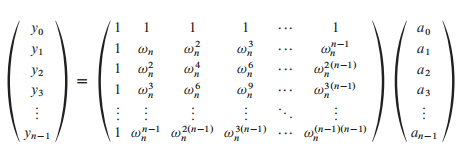
\includegraphics[scale = 0.6]{2.png}
          \newline
          可验证, 上述矩阵的逆为$A^{-1}_{i, j} = {\omega_n^{-ij} / n}$
        \item DFT的逆运算为$a_j = \frac{1}{n}\sum\limits_{k = 0}^{n - 1}y_k\omega_n^{-kj}$, 这也是多项式求值的形式, 也可以用$\Theta(n\log n)$的时间完成.
        \item 算法导论中还介绍了一种常数更低的实现方式.
      \end{itemize}
    \end{frame}

\section{convex hull}
  \subsection{intro. and algo.}
    \begin{frame}
      \frametitle{convex hull-intro. and algo.}
      \begin{itemize}
        \item 问题$\ \ $给定离散点集, 求最小的凸多边形包含所有点
        \pause \item 算法
          \begin{itemize}
            \item 以$y_{max}, y_{min}$的连线分成两个点集
            \item $deal(L)$
              \begin{itemize}
                \item 将距离分界线最远点加入凸包, 连接两条新分界线
                \item 考虑用新分界线划分成的两个新子问题
              \end{itemize}
            \item $deal(R)$
          \end{itemize}
      \end{itemize}
    \end{frame}

  \subsection{analysis}
    \begin{frame}
      \frametitle{algorithm analysis}
      \begin{itemize}
        \item 初始用直线分割  O(n)
        \item $deal(n)$的复杂度  $W(n) \leq W(n - 1) + O(n)$
          \begin{itemize}
            \item 找距离最远点   $O(n)$
            \item 找三角形外面的点 $O(n)$
            \item 新的子问题至多只有$n - 1$个点
          \end{itemize}
        \item $T(n) = O(n) + W(n) = O(n^2)$
      \end{itemize}
    \end{frame}
\section{other problems}
  \begin{frame}
    \frametitle{other problems}
    \begin{itemize}
      \item 二分查找  $\quad \  T(n) = T(n / 2) + \Theta(1)$
      \item 棋盘覆盖
        \begin{equation*}
          T(n) = \left\{
          \begin{aligned}
            & O(1) & k = 0 \\
            & 4T(k - 1) + O(1) & k > 0 \\
          \end{aligned}
          \right.
        \end{equation*}
      \item 幂的和 $\quad \quad \  T(n) = T(n / 2) + \Theta(1)$
    \end{itemize}
  \end{frame}
\end{CJK*}
\end{document}
